%フォーマット更新日:20210728
%
%

\documentclass[10pt,onecolumn]{jsarticle}

\usepackage[dvipdfmx]{graphicx}
\usepackage{multirow}
\usepackage{url}
\usepackage{otf}
\usepackage{here}
\usepackage{bm}
\usepackage{amsmath}
\usepackage{algorithmic}
\usepackage{algorithm}

\renewcommand{\refname}{次に読むべき論文のリスト}


\newcommand{\hama}{\ajMayuHama}


\pagestyle{empty}

\setlength{\topmargin}{6mm}
\setlength{\oddsidemargin}{-4mm}
\setlength{\evensidemargin}{-4mm}
\setlength{\textwidth}{175mm}
\setlength{\headsep}{0pt}
\setlength{\headheight}{0pt}
\setlength{\textheight}{235mm}
\setlength{\columnsep}{5mm}

\begin{document}

%\twocolumn[%
\vspace{-20mm}
\begin{center}
{\LARGE\textbf{論文メモ}}
\end{center}

\begin{flushright}
\begin{tabular}{|c|l|}
%\hline
%版数  &   0001からはじめる
%\\
\hline
文献番号  &  0016
\\
\hline
日付  &  2021年01月21日
\\
\hline
名前  &  武川海斗
\\
\hline
\end{tabular}
\end{flushright}
%]

%--------------
%本文開始
%--------------

%-------------------------------------------------------------------------
%\section*{論文情報}
%-------------------------------------------------------------------------
%
%論文の基本情報についてまとめる
%
\begin{center}
{\large 文献情報}
\begin{table}[hbp]%[H]
\begin{tabular}{|l||l|}
\hline
著者  &  R. R. Yager and D. P. Filev
\\ \hline
英文タイトル  & Approximate Clustering Via the Mountain Method
\\ \hline
和文タイトル  & マウンテン法による近似クラスタリング
\\ \hline
書誌情報  &  IEEE TRANSACTIONS ON SYSTEM,Vol.~24,No.~8,pp.~1279--1284(ページ),1994
\\ \hline
キーワード &
\\ \hline
\end{tabular}
\end{table}
\end{center}

\section{論文のトピック}
本論文は,ファジィ$c$-meansの中心を推定する手法として,マウンテンクラスタリングを提案している.
マウンテンクラスタリングとは,データ空間を格子状で与え,格子状の座標とデータの距離に基づき値を与える手法である.

\section{ベースとなった手法}
\subsection{ファジィ$c$-means}
ファジィ$c$-meansはクラスター中心と帰属度について交互最適化を行うことでクラスタリングを行う.
\begin{align}
	J_{m}=\sum_{k=1}^{n} \sum_{i=1}^{q} v_{i k}^{m}\left|x_{k}-x_{i}\right|^{m}
\end{align}
データ数を$n$,クラスタ数を$q$とし,$v_{ik}$はクラスタ$i$に属するデータ$k$を表す.また,$x_i$はクラスタ中心である.

\section{提案手法のコア要素}
\subsection{マウンテンクラスタリング}
マウンテンクラスタリングは,データ空間を格子状で表し格子の頂点とデータの距離から算出した値を与える.この値をM値とし,以下の式で与える.M値が高いほど,データの格子の頂点にデータが集まっていることを表す.
\begin{align}
	M\left(N_{i}\right)=\sum_{k=1}^{n} e^{-\alpha d\left(x_{k}, N_{i}\right)}
\end{align}
ここで,$N_i$ はi個目の格子の頂点を表し,$\alpha$はパラメータである.
$(x_k, N_i)$は,データkと格子の頂点$N_i$との距離を表す.$M(N_{i})$は$N_i$の周りにデータがあるほど高い値を示す.マウンテンクラスタリングでは,M値が大きい格子の頂点をクラスタの中心とする.
最も大きいM値は,以下の式で選択される.
\begin{align}
	M_{1}^{*}=\operatorname{Max}_{i}\left[M\left(N_{i}\right)\right]
\end{align}
ここで,k番目に大きなM値は以下の式で表される.
\begin{align}
	\widehat{M}^{k}\left(N_{i}\right)=\widehat{M}^{k-1}\left(N_{i}\right)-M_{k-1}^{*} \sum_{k=1}^{n} e^{\beta d\left(N_{k-1}^{*}, N_{i}\right)}
\end{align}
子の頂点を表す.なお,$\beta$はパラメータである.一度選択された格子の頂点の影響を考慮し,第二項でk−1番目に大きいと選択された格子の頂点と$N_i$のM値を引く.
例えば,2番目に大きなM値を持つ格子の頂点は,一番大きな格子の頂点の影響を取り除いて選択される.大きなM値を持つ格子の頂点の周りも大きなM値を持っており,各クラスタ中心の推定に影響があるため,前回選択された格子の頂点の影響を取り除く.
\section{実験デザイン・結果と考察}
実験では,2次元で表される 10個のデータに対してmountainクラスタリングを用いた図(\ref{figure}).
格子の数は各次元でそれぞれ6個に分けられる.パラメータは,$\alpha = \beta = 5.4$ とした.クラスタ中心の選択は,最も大きなM値を持つ格子の頂点とk−1番目に大きなM値の比率を計算し,一定の値以下になるまで行なった.
実験の結果,良好なクラスタリングを行うことができた.
	\begin{figure}
		\label{figure}
	\centering
	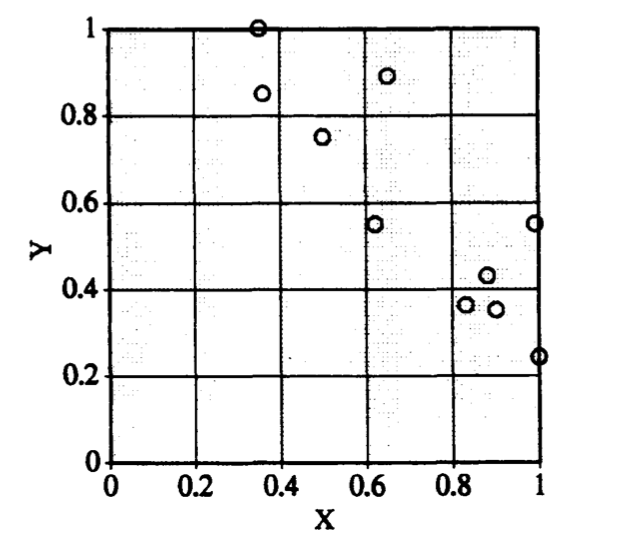
\includegraphics[width=5cm]{figure.png}
	\caption{実験データ}
\end{figure}
\section{手法の限界・今後の課題}
この手法は,高次元なデータに対して分類を行うことが困難であることが述べられている.高次元になれば,格子点を求めることが困難になるからで,計算量も激増する.



%%%%%%%%%%%%%%%%%%%%
%%%%%%%%%%%%%%%%%%
\end{document}
